\chapter{Implementacja}\label{chap:impl}
{
    Do implementacji wymaganych narzędzi oraz funkcjonalności skorzystano z języka Python. Głównym powodem tłumaczącym wybór tego języka programowania jest jego prostota, przenośność oraz szeroki zbiór wysokopoziomowych bibliotek często opartych na wydajnych implementacjach algorytmów napisanych w językach niskiego poziomu, takich jak C i C++. 

    Kolejną zaletą języka Python jest dostępność systemu zarządzania bibliotekami - {\textit {pip}}, oraz narzędzi kontrolujących środowisko uruchomieniowe gwarantujące użycie poprawnej wersji interpretera i zależności na różnych systemach - {\textit {pipenv}}. Dodatkowo, wykorzystano popularne w dziedzinie analizy danych środowisko zastępujące standardowy interaktywny interpreter - {\textit {Jupyter Notebook}}. Pozwala ono między innymi na jednoczesną wizualizację i tworzenie procesu przetwarzania danych. 

    \section{Wykorzystane biblioteki}
    {
        Podczas implementacji projektu, korzystano z następujących bibliotek programistycznych:
        \begin{itemize}
            \setlength\itemsep{-0.5em}
            \item Tensorflow - biblioteka umożliwiająca przeprowadzanie zaplanowanych procesów obliczeń na tensorach, będących fundamentem procesu uczenia sieci neuronowych. Podczas pracy skorzystano z wysokopoziomowego interfejsu tensorflow.keras, zawierającego predefiniowane architektury i warstwy sieci. Za pomocą interfejsu biblioteki możliwe było utworzenie oraz uczenie modelu o architekturze opisanej w rozdziale \ref{chap:main-model}.
            \item numpy - biblioteka rozszerzająca funkcjonalność języka Python o wydajne i łatwe w obsłudze operacje numeryczne na n-wymiarowych tablicach. Zastosowanie biblioteki miało miejsce w procesie opracowania danych. Dodatkowo, przetworzone dane były zapisywane na dysk w formacie natywnym dla biblioteki numpy, ponieważ modele utworzone za pomocą narzędzia Tensorflow przystosowane są do współpracy z takim rodzajem danych.
            \item mido - biblioteka służąca do dekodowania plików w formacie midi. Umożliwia wczytywanie plików z dysku oraz odczyt zdarzeń zapisanych na poszczególnych ścieżkach pliku. Uzyskane zdarzenia posiadają wszystkie niezbędne atrybuty, takie jak: rodzaj wiadomości, wysokość dźwięku oraz ilość jednostek czasu które upłynęły od poprzedniego zdarzenia.
            \item scipy - biblioteka zawierająca implementację algorytmu k-Means użytego w procesie grupowania wartości rytmicznych dźwięków (\ref{sec:group_rythm}).
            \item gensim - biblioteka zawierająca implementację modelu Word2Vec wymaganego do wyznaczenia wektorów zanurzonych (\ref{sec:embed}).
        \end{itemize}
    }

    \section{Specyfikacja zewnętrzna}
    {
        Korzystanie z dostępnych metod obróbki danych umożliwiają skrypty znajdujące się w folderze {\textit {{scripts}}}. Z powodu chęci zachowania jak największej elastyczności i możliwości wielokrotnego używania tego samego kroku procesu, wynikiem działania części skryptów są dane w postaci pośredniej lub metadane konieczne w innych krokach procesu.

        Poniższa lista zawiera opis poszczególnych skryptów oraz ich przypadków użycia:
        \begin{itemize}
            \setlength\itemsep{-0.5em}
            \item {\textbf {create\_sparse\_notes\_sampled\_time.py}} - przeprowadza transformację plików midi do postaci w której dźwięki są reprezentowane za pomocą kodu M\,\,z\,\,N a upływ czasu poprzez próbkowanie (postać opisana w rozdziałach \ref{sec:note-codes} i \ref{sec:samle_time}). Do parametrów wywołania należy folder plików źródłowych, folder docelowy oraz okres próbkowania. Możliwe jest również przeprowadzenie transformacji odwrotnej.
            \item {\textbf {create\_sparse\_clustered\_time.py}} - transformuje pliki midi do postaci kodu M\,\,z\,\,N z grupowaną wartością rytmiczną (\ref{sec:note-codes} i \ref{sec:group_rythm}). Podczas pracy skryptu uczony jest model k-Means odpowiedzialny za wyznaczenie zadanej ilości grup wartości rytmicznych. Parametrami wejściowymi jest folder źródłowy, folder docelowy oraz kierunek transformacji.
            \item {\textbf {prepare\_for\_embedding.py}} - jako dane wejściowe przyjmuje utwory w których informacja o wysokości dźwięku jest wyrażona za pomocą kodu M\,\,z\,\,N i generuje metadane konieczne do przeprowadzenia procesu wyznaczania wektorów zanurzonych (\ref{sec:embed}). Do tworzonych danych należy przekształcony zbiór wejściowy pozbawiony powtórzeń bezpośrednio następujących po sobie dźwięków, słownik zawierający występujące w zbiorze wielodźwięki oraz ich liczność. 
        \end{itemize} 

        Pełną listę argumentów każdego z skryptów można uzyskać poprzez jego uruchomienie z flagą {\textit {--help}}.

        W przypadku procesów których automatyzacja była kłopotliwa lub istotna była wizualizacja przebiegu zadania, skorzystano z plików {\textit {Jupyter Notebook}}.

        Do najistotniejszych należą:
        \begin{itemize}
            \setlength\itemsep{-0.5em}
            \item {\textbf {{Word2Vec.ipynb}}} - zawiera proces uczenia modelu Word2Vec służącego do wyznaczania wektorów zanurzonych odpowiadających zapisowi M\,\,z\,\,N wielodźwięków. Umożliwia ręczne ustalenie ilości koniecznych powtórzeń uczenia na podstawie postępu treningu. Wynikiem działania procesu jest plik zawierający mapowanie konkretnych wielodźwięków na wektory zanurzone.
            \item {\textbf {{LSTM\_clustered\_time\_sparse.ipynb}}} - zawiera proces uczenia sieci neuronowej za pomocą danych w postaci kodu M\,\,z\,\,N i grupowanych wartości rytmicznych. W trakcie uczenia oraz po jego zakończeniu możliwe jest zapisanie modelu na dysk.
            \item {\textbf {{LSTM\_clustered\_time\_with\_embedded.ipynb}}} - rozszerza funkcjonalność powyższego procesu o etap konwersji danych wejściowych do postaci w której wysokości dźwięków są w postaci wektorów zanurzonych. Konieczne jest wskazanie pliku wygenerowanego za pomocą procesu {\textit {{Word2Vec.ipynb}}}.
            \item {\textbf {LSTM\_generating\_clustered\_time\_embedded.ipynb}} - zawiera proces generacji i transformacji próbek do postaci plików midi. Wymaga wskazania ścieżki do pliku modelu sieci neuronowej oraz słownika wektorów zanurzonych.
            \item {\textbf {{MeasuringDataset.ipynb}}} - przeprowadza proces wyznaczania miar opisujących zbiór danych treningowych. Miary zostały opisane w rozdziale \ref{sec:measuremnts}.
            \item {\textbf {{MeasuringGenerated.ipynb}}} - przeprowadza proces wyznaczania miar dla wygenerowanych próbek za pomocą wskazanego modelu. 
        \end{itemize}
    }

    \section{Specyfikacja wewnętrzna}
    {
        Kod źródłowy został podzielony na moduły odpowiadające za poszczególne funkcjonalności projektu. Lista modułów projektu:

        \begin{itemize}
            \setlength\itemsep{-0.5em}
            \item {\textbf {data\_processing}} 
            \item {\textbf {evaluation}}
            \item {\textbf {training}}
            \item {\textbf {generating}}
        \end{itemize}

        Strukturę projektu przedstawia rysunek \ref{folder_struct}.

        \begin{figure}
            \centering
            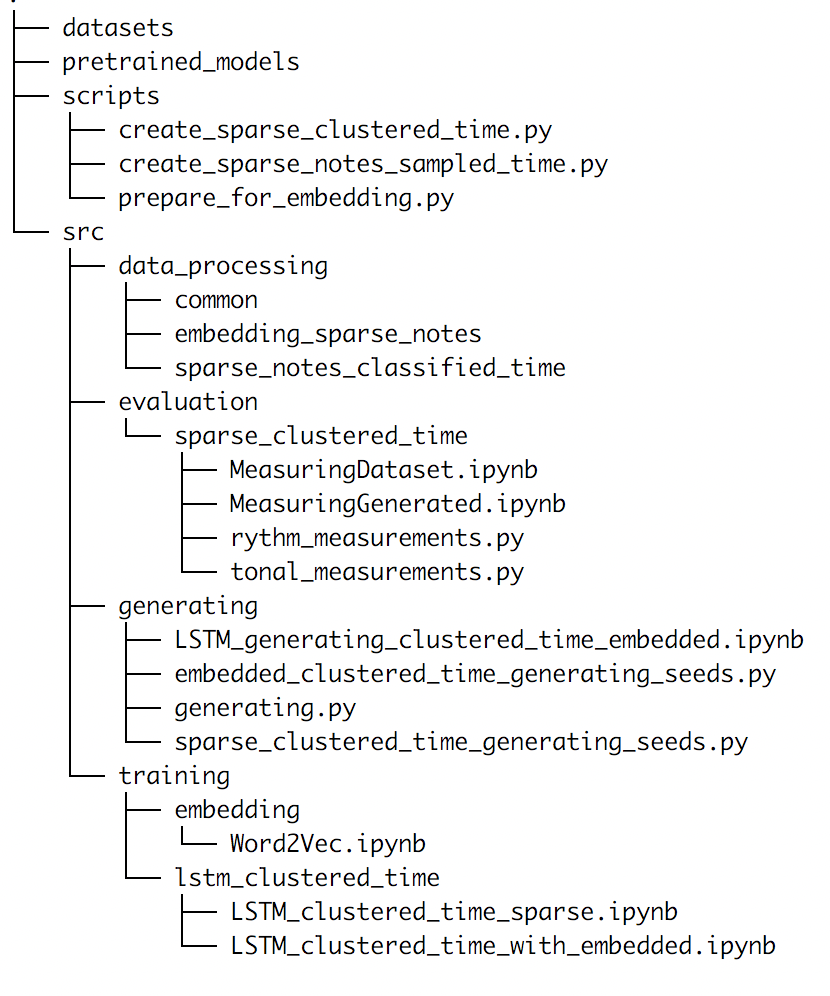
\includegraphics[scale=0.7]{folder_struct}
            \caption{Hierarchia folderów i modułów projektu}
            \label{folder_struct}
        \end{figure}

        \subsection{Moduł data\_processing}
        {
            Zawiera definicje funkcji odpowiedzialnych za przetwarzanie danych w postaci plików midi do postaci numerycznej i z numerycznej do midi. Moduł został podzielony na podfoldery ze względu na rodzaj numerycznej reprezentacji danych. Zaimplementowane w module metody umożliwiają uzyskanie danych w postaci:
            \begin{itemize}
                \setlength\itemsep{-0.5em}
                \item Kod  M\,\,z\,\,N + próbkowanie
                \item Wektory zanurzone + próbkowanie
                \item Wektory zanurzone + czas jako zmienna ciągła
                \item Kod  M\,\,z\,\,N + pogrupowane długości dźwięków
                \item Wektory zanurzone + pogrupowane długości dźwięków
            \end{itemize}


        }

        \subsection{Moduł evaluation}
        {
            Zawiera miary opisane w rozdziale \ref{sec:measuremnts}. Funkcje wyznaczające wartości miar przystosowane są do współpracy z danymi wejściowymi w postaci kodu M\,\,z\,\,N dla wysokości dźwięków oraz kodu 1\,\,z\,\,N w przypadku informacji o czasie jego trwania. Oznacza to, że w celu dokonania pomiarów próbek w których wysokości dźwięków opisują wektory zanurzone, konieczne jest uprzednia transformacja przy użycia słownika uzyskanego za pomocą modelu Word2Vec.
        }

        \subsection{Moduł training}
        {
            Główną zawartością modułu są {\textit {Notebooki}} służące do uczenia modeli, przeznaczone do uruchomienia lokalnie lub w usłudze Google Colab. 
        }

        \subsection{Moduł generating}
        {
            Zawiera funkcje konieczne do przeprowadzenia procesu generacji próbek będących w postaci danych opracowanych w module {\textbf {data\_processing}}. W pliku {\textit {generating.py}} zawarto implementację głównej idei podejścia do procesu generacji próbek opisanej w rozdziale \ref{sec:gen_method}. W pozostałych plikach modułu zdefiniowano funkcje ziaren służących do początkowania procesu generowania. Ziarna podzielono ze względu na wewnętrzną postać danych.
        }

    }

    \section{Walidacja kodu}
    {
        Duża część modułu {\textit {data\_processing}} oraz {\textit {evaluation}} została pokryta testami jednostkowymi sprawdzającymi poprawność ich implementacji. 
        Testy okazały się pomocnym narzędziem, które pozwoliło wcześnie dostrzec błędy w logice aplikacji.

        Do implementacji testów wykorzystano bibliotekę {\textit {unittest}}.
    }

    \pagebreak

    \section{Uruchamianie}
    {
        Do uruchomienia narzędzi konieczne jest posiadanie interpretera języka Python, menadżera zależności {\textit {pip}} oraz środowiska {\textit {pipenv}}. Po wykonaniu poniższej komendy w głównym katalogu projektu, powinna zostać uruchomiona konsola w środowisku zawierającym wszystkie wymagane zależności.

        \begin{verbatim}
            pipenv install && pipenv shell
        \end{verbatim}

        Z uruchomionej konsoli można uruchomić serwer {\textit {Jupyter}}, wykonać skrypt lub uruchomić konsolę interpretera języka Python.


        Poniżej przedstawiono przykładowe użycie skryptu \\{\textit {create\_sparse\_clustered\_time.py}}:
        \begin{verbatim}
            python scripts/create_sparse_clustered_time.py 
                --mode=mid2np 
                --src=./path/to/midi 
                --dst=./output
        \end{verbatim}
    }
}